\documentclass[4pt,a4papper]{article}
\usepackage{ctex}  
\usepackage{amsmath}
\usepackage{mathtools}
\usepackage{upgreek}
\pagestyle{headings}
\usepackage{graphicx}
\usepackage{subfigure}
\usepackage{indentfirst}
\usepackage{fancyhdr}
\usepackage{listings}
\usepackage{amsmath}
\usepackage{longtable}
\usepackage{geometry}
\usepackage[usenames,dvipsnames]{color}
\definecolor{lightgray}{RGB}{230,230,230}
\lstset{ language=, numbers=left, basicstyle=\small,
  keywordstyle=\color{blue}, commentstyle=\color{PineGreen},
  stringstyle=\color{red}, frame=shadowbox, breaklines=true,
  backgroundcolor=\color{lightgray},extendedchars=false }


\geometry{left=1.5cm,right=1.5cm,top=3cm,bottom=1.5cm}

%opening
\title{\zihao{-2}\textbf{最大气泡压力法实验报告}}
\author{张锦程}
\date{\today}

\begin{document}
\maketitle
%\tableofcontents

\section{\zihao{4}实验目的}
1.测定不同浓度正丁醇溶液的表面张力。

2.根据吉布斯公式计算正丁醇溶液的表面吸附量。

3.掌握用最大气泡法测定表面张力的原理和技术。

\section{\zihao{4}实验原理}
液体表面层的分子受内层分子的吸引与受表面层外介质的吸引并不相同,处于不平衡状态,具有较大势能,如欲使液体产生新的表面,就需要对其做功。可逆地使表面积增加 $dA$ 所需作的功为$-\delta W = ydA,(1)$ 

比例系数 $y$ 表示在等温等压下形成单位表面所需的可逆功,其数值等于作用在界面上每单位长度边缘的力,称为表面张力。\

纯液体降低表面自由能的唯一途径是尽可能缩小其表面积。对于溶液,由于溶质使溶剂表面张力发生变化,因此可以调节溶质在表面层的浓度来降低表面自由能。根据能量最低原则,溶质能降低溶剂的表面张力时,表面层溶 质的浓度比溶液内部大;反之,溶质使溶剂的表面张力升高时,表面层溶质的浓度比内部的浓度低(溶液的表面吸附)。 它们之间的关系遵守吉布斯公式∶$\Gamma = -\frac{c}{RT}\frac{d\gamma}{dc}_{T_p} (2)$ 式中∶$\Gamma$ 为表面吸附量$(mol·m²),y$ 为表面张力$(N·m²)$ 

本实验采用最大气泡法测定表面张力。降低毛细管外压力,则气泡将自管口内壁逐渐形成,见下图。开始时形成的气泡曲率半径很大,随后半径逐渐变小, 泡内外的压力差逐渐增加。当形成的气泡刚好是半球形时半径最小,泡内外压力差达到最大值。此后半径又逐渐变大,压力差逐渐下降,从而使气流冲入气泡内最终将其吹离管口。在此过程中,最大压力差记为$\Delta p$,气泡呈半球形时的半径为 $r$,由 Young-Laplace 方程有:$\Delta p = 2\frac{\gamma}{r}, \gamma = \frac{r\Delta p}{2}; \frac{\gamma_1}{\gamma_2} = \frac{\Delta h_1}{\Delta h_2}; \gamma_1 = \frac{\Delta h_1 \gamma_2}{\Delta h_2} = K\Delta h_1$ 

式中的 $K$ 值对同一支毛细管及同一种压力计介质是常数,称作仪器常数。由已知表面张力的液体作标准求出常数 $K$

\section{\zihao{4}实验操作}
1.溶液配制

用容量瓶及所给正丁醇水溶液配制浓度分别为 0.3、0.25、0.2、0.15、0.1、0.05、0.025 $mol·dm^{-3}$ 的正丁醇水溶液。

2.测定仪器常数

充分洗净大试管 4 及毛细管 1,在大试管中注入适量的去离子水,使毛细管端口刚好和液面垂直相切。 将大试管安装在恒温水浴内,给抽气瓶 3 注满水。当温度恒定后打开抽气瓶的活塞,使瓶内的水缓慢滴出,使大试管逐步减压,在毛细管 1 的端口形成气泡。调节抽气瓶水流速,使气泡均匀产生,形成速度控制在不少于 10~20 秒一个。读出气泡脱离毛细管端口瞬间 U 型压力计液面的高度差,准确读取 3 次,求平均值,得 $\Delta h_2$ 。查出该温度的 $\gamma_2$ (水的表面张力)值, 由 7 式可求出仪器常数 $K$ 值。

3.测定正丁醇溶液的表面张力

同样方法,分别测定不同浓度 $(0.025 \sim 0.5 mol·dm^{-3})$正丁醇溶液的 $\Delta h$ 值。每次测量前,先将大试管和毛细管用去离子水洗净,再用被测液润洗 $2 \sim 3$ 次,注意毛细管端口勿使其碰损。



\section{\zihao{4}实验结果讨论}
\subsection{\zihao{-4}计算处理过程}
1.求出各浓度正丁醇水溶液的 $\gamma$。 

2.在坐标纸上作 $\gamma - c$ 图(曲线要光滑),在曲线上取 6~7 个点,用镜面法作切线,求出 Z 值。

3.由 $\Gamma = Z/RT$ 计算不同浓度溶液的 $\Gamma$ 值,并计算出 $c/\Gamma$ 值。

4.作“$\frac{c}{\Gamma} - c$”图,由直线斜率求出 $\Gamma_{\infty}$

\subsection{\zihao{-4}测定结果}
    \begin{figure}[htbp]
        %\small
        \centering
        \includegraphics[width=12cm]{./figures/水.png}
        \caption{Figure 1:水的参比值} \label{fig:1}
    \end{figure}

    \begin{figure}[htbp]
        %\small
        \centering
        \includegraphics[width=12cm]{./figures/0_025.png}
        \caption{Figure 2:正丁醇浓度:0.025 $mol·dm^{-3}$} \label{fig:2}
    \end{figure}

	\begin{figure}[htbp]
        %\small
        \centering
        \includegraphics[width=12cm]{./figures/0_05.png}
        \caption{Figure 3:正丁醇浓度:0.05 $mol·dm^{-3}$} \label{fig:3}
    \end{figure}

	\begin{figure}[htbp]
        %\small
        \centering
        \includegraphics[width=12cm]{./figures/0_10.png}
        \caption{Figure 4:正丁醇浓度:0.10 $mol·dm^{-3}$} \label{fig:4}
    \end{figure}

    \begin{figure}[htbp]
        %\small
        \centering
        \includegraphics[width=12cm]{./figures/0_15.png}
        \caption{Figure 5:正丁醇浓度:0.15 $mol·dm^{-3}$} \label{fig:5}
    \end{figure}

    \begin{figure}[htbp]
        %\small
        \centering
        \includegraphics[width=12cm]{./figures/0_20.png}
        \caption{Figure 6:正丁醇浓度:0.20 $mol·dm^{-3}$} \label{fig:6}
    \end{figure}

    \begin{figure}[htbp]
        %\small
        \centering
        \includegraphics[width=12cm]{./figures/0_25.png}
        \caption{Figure 7:正丁醇浓度:0.25 $mol·dm^{-3}$} \label{fig:7}
    \end{figure}

    \begin{figure}[htbp]
        %\small
        \centering
        \includegraphics[width=12cm]{./figures/0_30.png}
        \caption{Figure 8:正丁醇浓度:0.30 $mol·dm^{-3}$} \label{fig:8}
    \end{figure}

    \begin{figure}[htbp]
        %\small
        \centering
        \includegraphics[width=12cm]{./figures/0_40.png}
        \caption{Figure 9:正丁醇浓度:0.40 $mol·dm^{-3}$} \label{fig:9}
    \end{figure}
\newpage

\subsection{\zihao{-4}讨论分析}
根据实验结果整理得下表:
\begin{table}[htbp]
\begin{tabular}{|l|l|l|l|l|l|l|l|l|l|}
\hline
\begin{tabular}[c]{@{}l@{}}正丁醇浓度单位:\\  $mol·dm^{-3}$\end{tabular} & 纯水(0.00) & 0.025  & 0.05   & 0.10   & 0.15   & 0.20   & 0.25   & 0.30   & 0.40   \\ \hline
电压值(mV)                                                           & 0.3799   & 0.3652 & 0.3438 & 0.3202 & 0.2662 & 0.2376 & 0.2268 & 0.2207 & 0.1952 \\ \hline
表面张力($10^{-2}N·m^{-1}$)                                           & 71.97    & 69.19  & 65.13  & 60.66  & 50.43  & 45.01  & 42.97  & 41.81  & 36.98  \\ \hline
\end{tabular}
\end{table}

使用对数函数对 $\gamma - c$ 曲线进行拟合后得到下图:
    \begin{figure}[htbp]
        %\small
        \centering
        \includegraphics[width=12cm]{./figures/lnfit_f.png}
    \end{figure}


\section{\zihao{4}结论}
在不同的位置做切线,计算 Z 和 $\Gamma$ ,求得“$\frac{c}{\Gamma} - c$”图如下:
    \begin{figure}[htbp]
        %\small
        \centering
        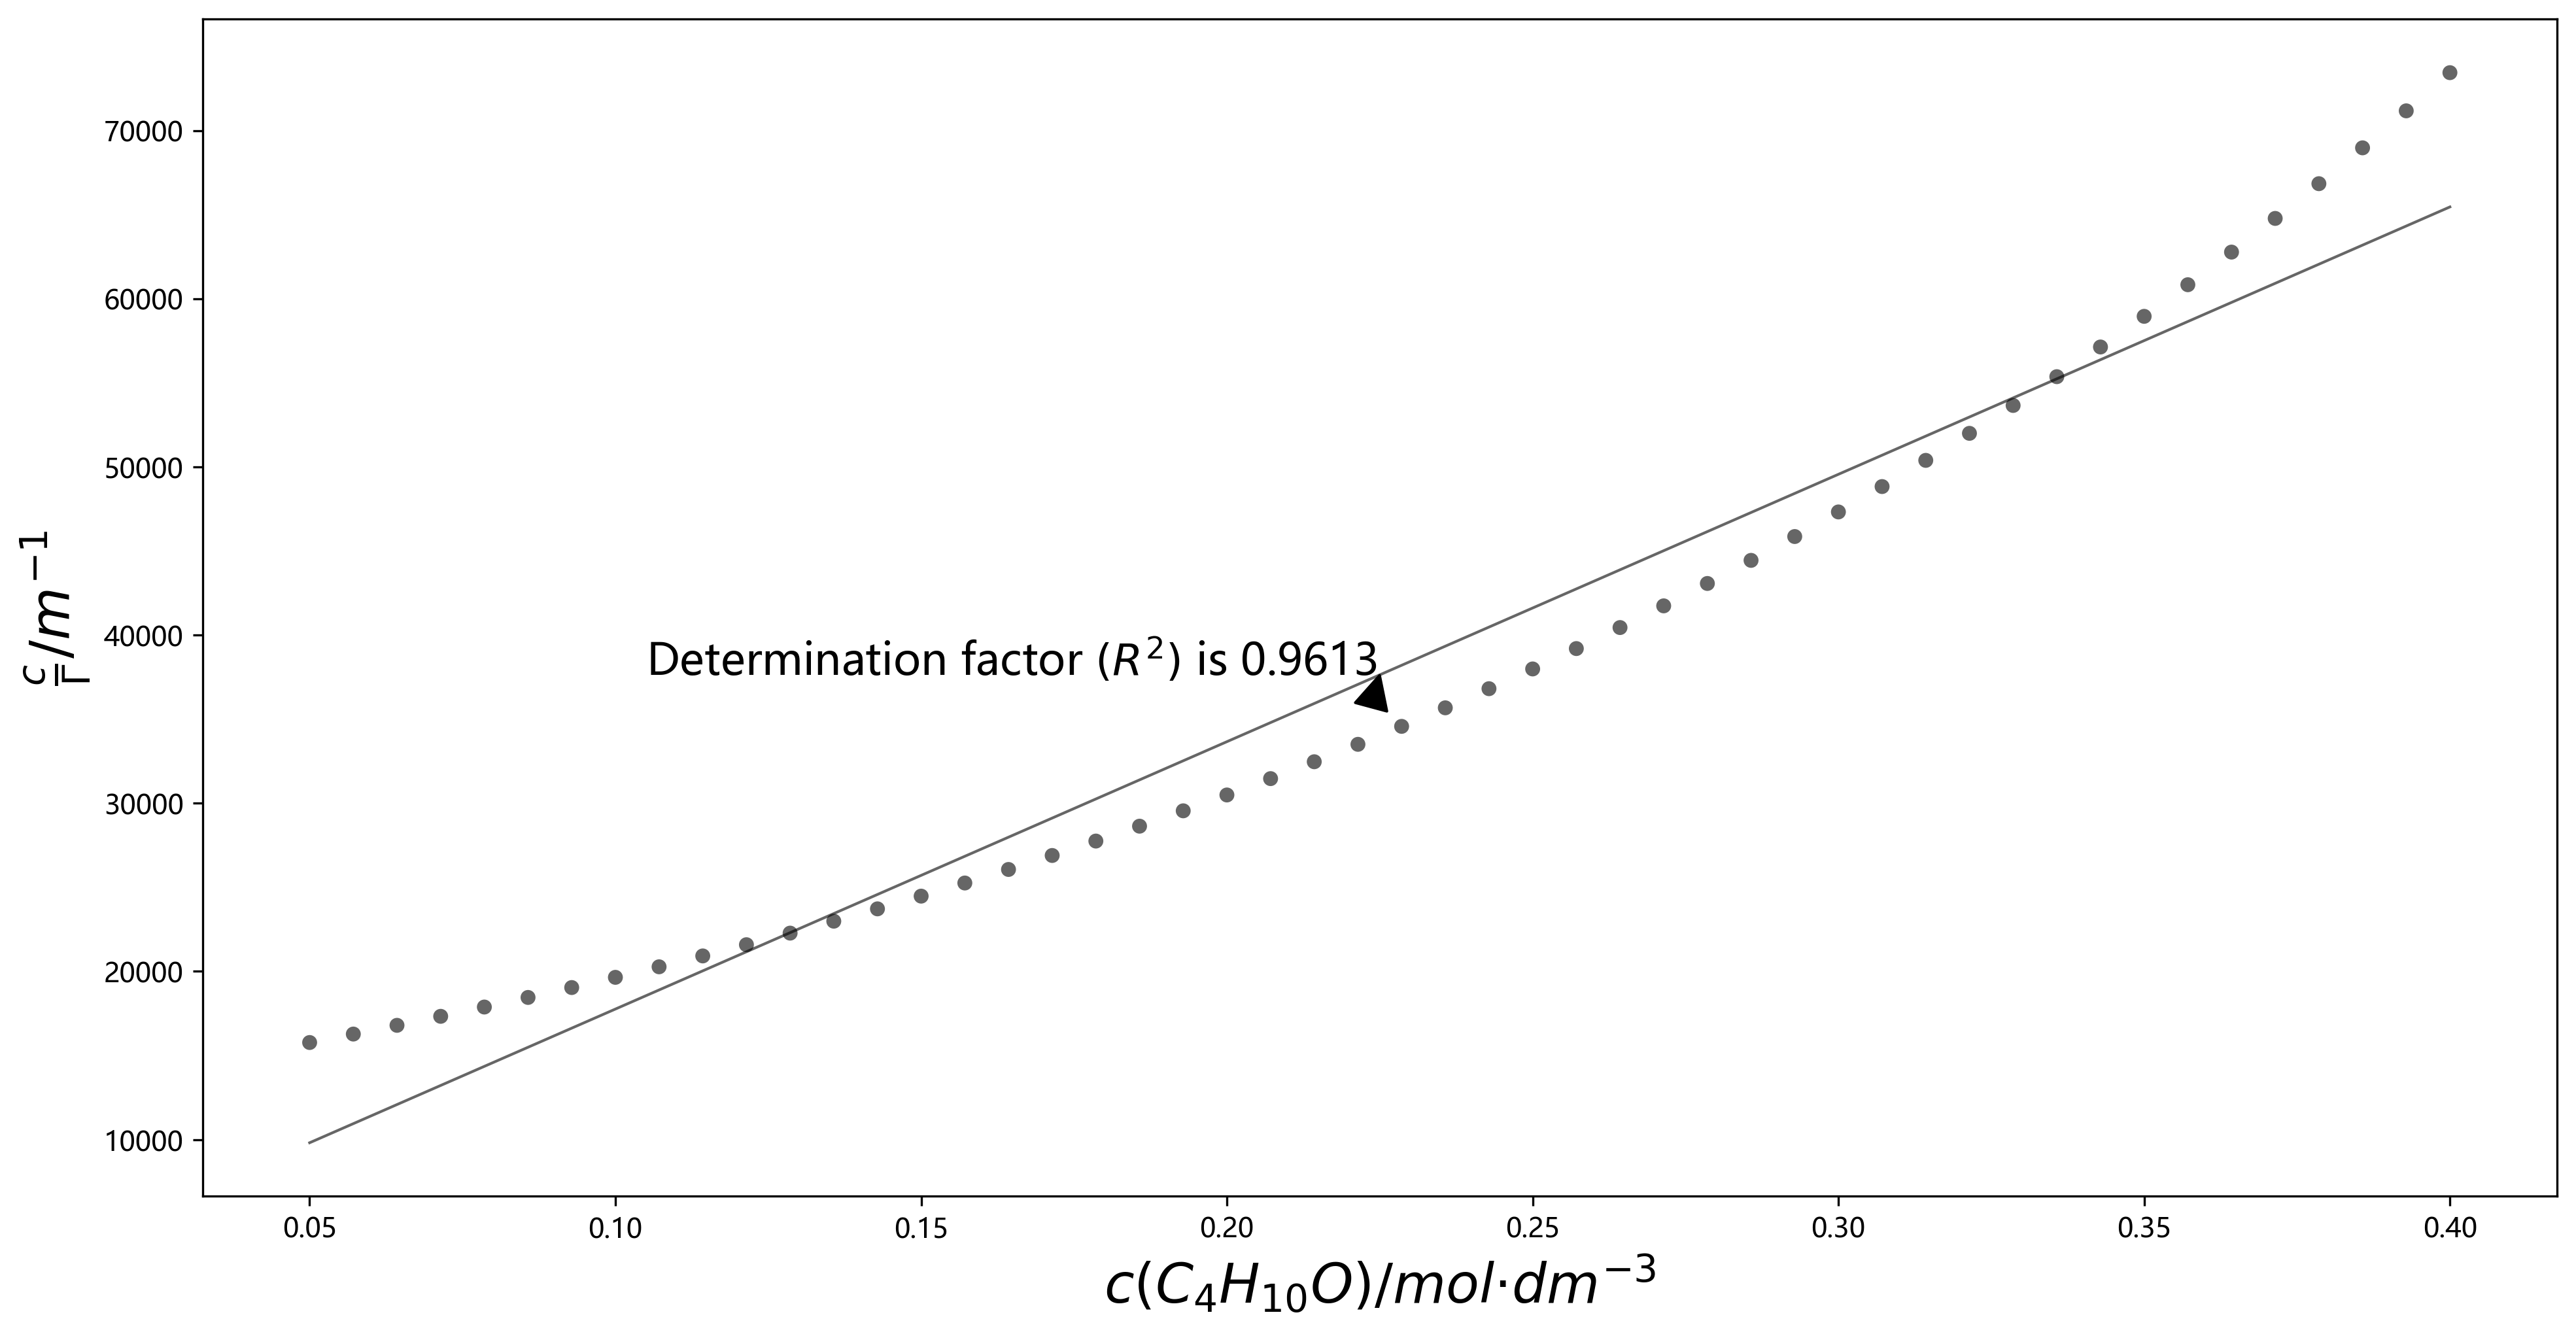
\includegraphics[width=12cm]{./figures/c_gamma_c.png}
    \end{figure}


线性拟合得到 $k = 158997.47 mol^{-1}·m^2$ 
求出 $\Gamma_{\infty} = \frac{1}{k} = 6.289 \times 10^{-6} mol·m^{-2}$



\newpage


\section{\zihao{4}附录}
\subsection{\zihao{-4}思考题}
1.要做好这个实验关键因素有哪些?

(1)毛细管垂直放置,其端口要和液面刚好接触,同时保证固定毛细管和外接装置的气密性,若密封度低,则气泡 溢出段不稳定,而且测得压力偏低。 
(2)仔细调节抽气瓶的滴水速度,出泡速度不可太快,否则不能达到平衡。 
(3)溶液配制要准确,按浓度从低到高的顺序测量。 
(4)表面张力对温度敏感,每次都应将溶液在恒温槽中静置一段时间,恒温后再测量。 

2.气泡形成速度过快对结果有何影响? 

会。若形成速度太快则可能会难以在压差最大点保持平衡(气泡破裂)。另外气泡的形成的短暂时间内是一个非稳态的过程,形成速度过快则可能对周围溶液产生扰动。若形成速度适中则可以有充分的时间建立平衡。 

3.为什么毛细管端口要和液面刚好接触?毛细管内径均匀与否对结果有无影响? 

如果毛细管深入液面下方太多,则测出的压差就包括了液面下方高度所产生的水压,导致了实验的误差。 无影响。实际上毛细管主体部分没有太大作用,主要起作用的是毛细管尖部分,主要应该保证端口处平整、半径均匀即可。


\clearpage
\end{document}